\documentclass[tikz,border=2pt]{standalone}

\usepackage{pgfplots,amsmath}
\pgfplotsset{compat=1.18}
\usetikzlibrary{shapes.geometric}
\usepgfplotslibrary{fillbetween}
\usepackage[colorlinks=true,linkcolor=blue,urlcolor=blue]{hyperref}

\begin{document}

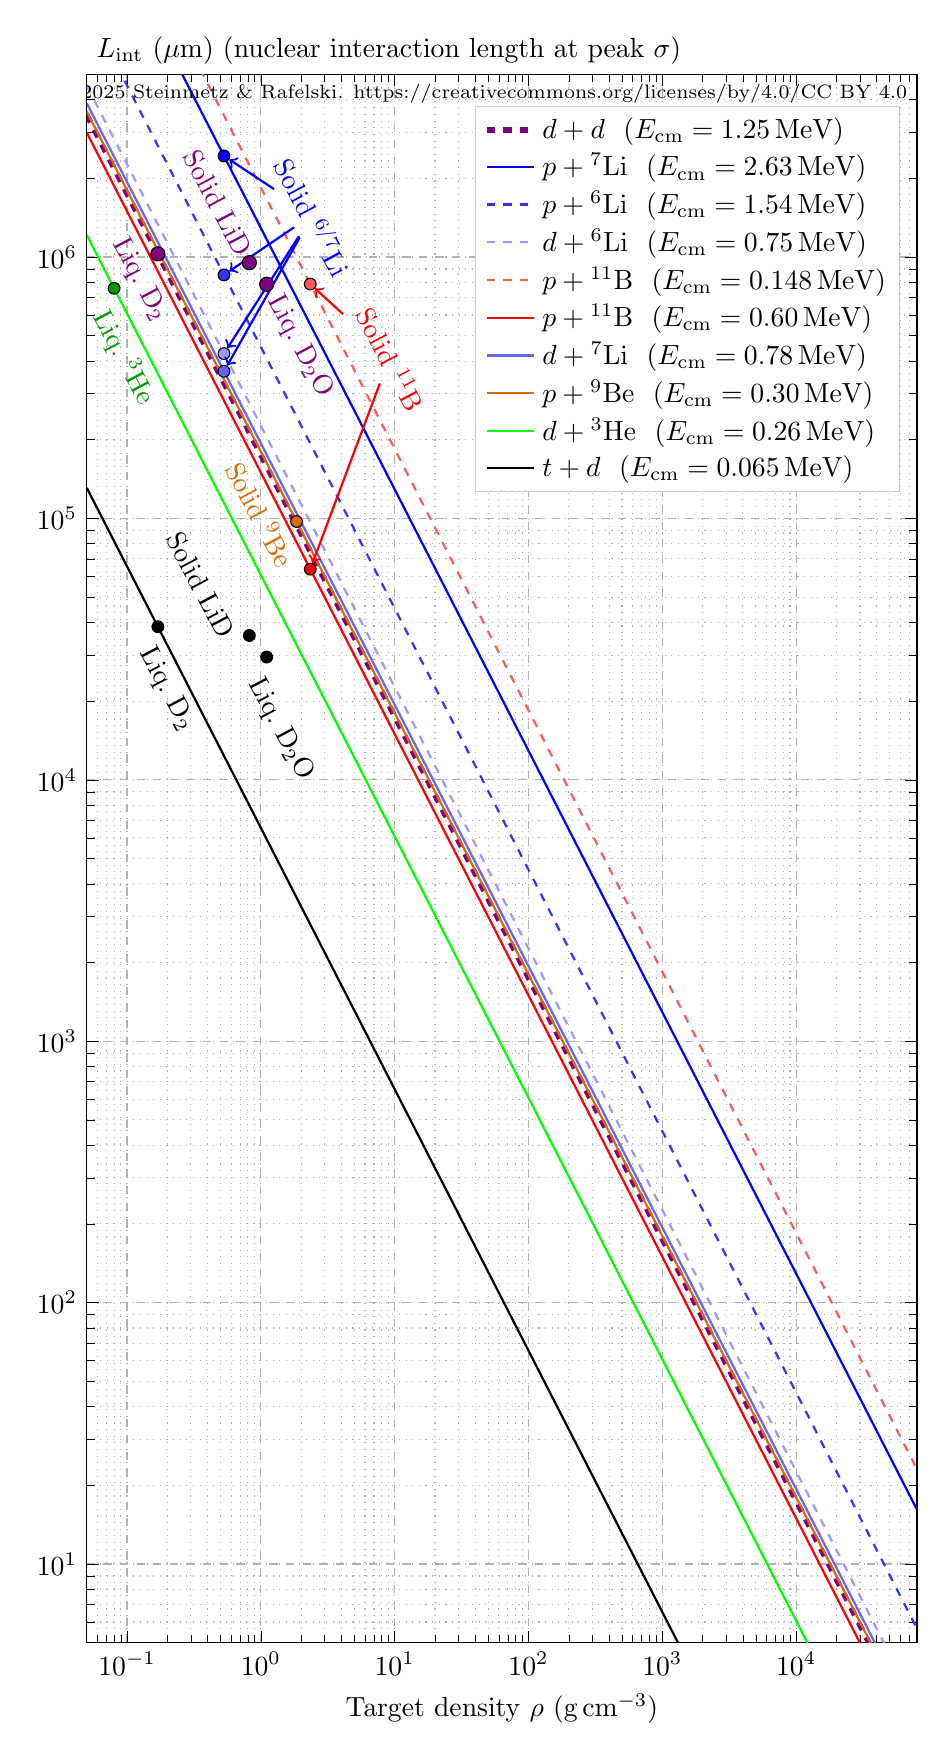
\begin{tikzpicture}

\def\Lscale{1e4}
\def\XMin{5e-2}
\def\XMax{8e4}
\def\YMax{\Lscale*5e2}
\def\YMin{\Lscale*5e-4}

%%%%%%%%%%%%%%%%%%%%%%%%%%%%%%%%%%%%%%%%%%%%%%%%%%%%%%%%%%%%%%%%%%%%%%%%%%%%
% Peak fusion cross-sections, summed over all exothermic (Q>0) exit channels of each entrance channel, evaluated at the c.m. energy where the sum peaks.
% m_areal = A_target / (N_A sigma) = 1.66054 * A_target / sigma[barn]  [g/cm^2]
%
%  channel   sigma[b]  E_cm[MeV]  E_lab[MeV]  channels summed / source
%  ---------------------------------------------------------------------------
%  d + d       0.19      1.25        2.50     d(d,p)t + d(d,n)3He; Bosch-Hale
%  t + d       5.07      0.065       0.162    d(t,n)alpha; Bosch-Hale
%  d + 3He     0.82      0.26        0.44     3He(d,p)alpha; Bosch-Hale
%  p + 6Li     0.22      1.54        1.80     6Li(p,3He)4He; Elwyn 1979 (EXFOR)
%  p + 7Li     0.09      2.63        3.00     7Li(p,alpha)4He; Cassagnou 1962
%  p + 9Be     0.83      0.30        0.33     9Be(p,alpha)6Li 0.36 b
%                                             + 9Be(p,d)8Be   0.47 b; Sierk 1973
%  p + 11B     1.22      0.60        0.655    11B(p,alpha_0+alpha_1); Becker 1987
%                                             broad 2- resonance,  12C* 16.57  MeV
%  p + 11B     0.099     0.148       0.1615   11B(p,alpha_0+alpha_1); Becker 1987
%                                             narrow 2+ resonance, 12C* 16.106 MeV
%  d + 6Li     0.44      0.75        1.00     (d,alpha) 0.06 + (d,p_0+p_1) 0.09
%                                             + (d,n)7Be 0.10 + (d,t)5Li 0.19
%  d + 7Li     0.60      0.78        1.00     total exothermic yield, dominated
%                                             by (d,n)8Be and (d,n alpha)alpha
%%%%%%%%%%%%%%%%%%%%%%%%%%%%%%%%%%%%%%%%%%%%%%%%%%%%%%%%%%%%%%%%%%%%%%%%%%%%

\def\NAinv{1.66054}          % 1/N_A in g, i.e. A/(N_A sigma_barn) prefactor

% d + d, summed over both branches d(d,p)t and d(d,n)3He
\def\sigmaDD{0.19}
\pgfmathsetmacro{\mArealDD}{\NAinv*2/\sigmaDD}
% t + d on a deuterium target
\def\sigmaTD{5.07}
\pgfmathsetmacro{\mArealTD}{\NAinv*2/\sigmaTD}
% d + 3He on a 3He target
\def\sigmaDHeThree{0.82}
\pgfmathsetmacro{\mArealDHeThree}{\NAinv*3/\sigmaDHeThree}
% p + 6Li
\def\sigmaPLiSix{0.22}
\pgfmathsetmacro{\mArealPLiSix}{\NAinv*6/\sigmaPLiSix}
% p + 7Li
\def\sigmaPLiSeven{0.09}
\pgfmathsetmacro{\mArealPLiSeven}{\NAinv*7/\sigmaPLiSeven}
% d + 6Li
\def\sigmaDLiSix{0.44}
\pgfmathsetmacro{\mArealDLiSix}{\NAinv*6/\sigmaDLiSix}
% d + 7Li
\def\sigmaDLiSeven{0.60}
\pgfmathsetmacro{\mArealDLiSeven}{\NAinv*7/\sigmaDLiSeven}
% p + 9Be, resonant alpha-producing channels sigma[p,alpha] + sigma[p,d]
\def\sigmaPBeNine{0.83}
\pgfmathsetmacro{\mArealPBeNine}{\NAinv*9/\sigmaPBeNine}
% p + 11B, broad 2- resonance at E_cm = 0.60 MeV
\def\sigmaPBEleven{1.22}
\pgfmathsetmacro{\mArealPBEleven}{\NAinv*11/\sigmaPBEleven}
% p + 11B, narrow 2+ resonance at E_cm = 0.148 MeV
\def\sigmaPBElevenNarrow{0.099}
\pgfmathsetmacro{\mArealPBElevenNarrow}{\NAinv*11/\sigmaPBElevenNarrow}

% Deuterium mass fractions of chemically bound targets
\def\wLiD{0.224}             % LiD
\def\wDtwoO{0.201}           % D2O

\begin{axis}[
  width=1.00\linewidth,
  height=21.5cm,
  xmode=log, ymode=log,
  xlabel={Target density $\rho$ (g\,cm$^{-3}$)},
  ylabel={$L_{\rm int}$ ($\mu$m) (nuclear interaction length at peak $\sigma$)},
  xmin=\XMin, xmax=\XMax,
  ymin=\YMin, ymax=\YMax,
  grid=both,
  major grid style={dashed,gray!60},
  minor grid style={dotted,gray!60},
  legend style={at={(0.98,0.98)},anchor=north east,fill=white,draw=gray!40,align=left},
  legend cell align=left,
  tick style={black},
  ylabel style={
    rotate=-90,
    at={(axis description cs:0,1.0)},
    anchor=south west,
    yshift=0pt}
]

% Curves (converted to microns)

% D + D (two branches: d(d,p)t and d(d,n)3He); color: violet
\addplot+[thick, no marks, domain=\XMin:\XMax, samples=400,
          color=violet, line width=2.0pt, dashed]
  ({x},{\Lscale*\mArealDD/x});

\addplot+[thick, no marks, domain=\XMin:\XMax, samples=400, color=blue, solid] ({x},{\Lscale*\mArealPLiSeven/x});
\addplot+[thick, no marks, domain=\XMin:\XMax, samples=400, color=blue!80, dashed] ({x},{\Lscale*\mArealPLiSix/x});
\addplot+[thick, no marks, domain=\XMin:\XMax, samples=400, color=blue!40, dashed] ({x},{\Lscale*\mArealDLiSix/x});
\addplot+[thick, no marks, domain=\XMin:\XMax, samples=400, color=red!65, dashed] ({x},{\Lscale*\mArealPBElevenNarrow/x});
\addplot+[thick, no marks, domain=\XMin:\XMax, samples=400, color=red, solid] ({x},{\Lscale*\mArealPBEleven/x});
\addplot+[thick, no marks, domain=\XMin:\XMax, samples=400, color=blue!60, solid] ({x},{\Lscale*\mArealDLiSeven/x});
\addplot+[thick, no marks, domain=\XMin:\XMax, samples=400, color=orange!85!black, solid] ({x},{\Lscale*\mArealPBeNine/x});
\addplot+[thick, no marks, domain=\XMin:\XMax, samples=400, color=green, solid] ({x},{\Lscale*\mArealDHeThree/x});
\addplot+[thick, no marks, domain=\XMin:\XMax, samples=400, color=black, solid] ({x},{\Lscale*\mArealTD/x});

\addlegendentry{$d + d$ \ ($E_{\rm cm}=1.25$\,MeV)}
\addlegendentry{$p + {}^{7}\textrm{Li}$ \ ($E_{\rm cm}=2.63$\,MeV)}
\addlegendentry{$p + {}^{6}\textrm{Li}$ \ ($E_{\rm cm}=1.54$\,MeV)}
\addlegendentry{$d + {}^{6}\textrm{Li}$ \ ($E_{\rm cm}=0.75$\,MeV)}
\addlegendentry{$p + {}^{11}\textrm{B}$ \ ($E_{\rm cm}=0.148$\,MeV)}
\addlegendentry{$p + {}^{11}\textrm{B}$ \ ($E_{\rm cm}=0.60$\,MeV)}
\addlegendentry{$d + {}^{7}\textrm{Li}$ \ ($E_{\rm cm}=0.78$\,MeV)}
\addlegendentry{$p + {}^{9}\textrm{Be}$ \ ($E_{\rm cm}=0.30$\,MeV)}
\addlegendentry{$d + {}^{3}\textrm{He}$ \ ($E_{\rm cm}=0.26$\,MeV)}
\addlegendentry{$t + d$ \ ($E_{\rm cm}=0.065$\,MeV)}

% Dots for condensed-phase densities (in microns)
\node[circle,fill=orange!85!black,draw=black,inner sep=1.5pt](BeNineDot)
  at (axis cs:1.85,{\Lscale*\mArealPBeNine/1.85}) {};
\node[anchor=north east,xshift=5pt,yshift=-15pt,rotate=-62,orange!85!black](BeNineLabel)
  at (axis cs:1.85,{\Lscale*\mArealPBeNine/1.85}) {\,Solid $^{9}$Be};

%\draw[thick,->,orange!85!black]
%  (BeNineLabel) -- (BeNineDot);

\node[circle,fill=red,draw=black,inner sep=1.5pt](BElevenDot)
  at (axis cs:2.34,{\Lscale*\mArealPBEleven/2.34}) {};

% Same solid-boron density on the narrow 0.148 MeV resonance curve
\node[circle,fill=red!65,draw=black,inner sep=1.5pt](BElevenNarrowDot)
  at (axis cs:2.34,{\Lscale*\mArealPBElevenNarrow/2.34}) {};

% One label serving both boron markers, arrows as for the Li family below
\node[anchor=south,xshift=22pt,yshift=-30pt,rotate=-62,red](BElevenLine)
  at (axis cs:2.34,{\Lscale*\mArealPBElevenNarrow/2.34}) {\,Solid $^{11}$B};

\draw[thick,->,red] (BElevenLine) -- (BElevenNarrowDot);
\draw[thick,->,red] (BElevenLine) -- (BElevenDot);

\node[circle,fill=green!60!black,draw=black,inner sep=1.5pt]
  at (axis cs:0.08,{\Lscale*\mArealDHeThree/0.08}) {};
\node[anchor=north west,rotate=-62,green!60!black] at (axis cs:0.08,{\Lscale*\mArealDHeThree/0.08}) {\,Liq.\ $^{3}$He};

\node[circle,fill=blue,draw=black,inner sep=1.5pt](LiDot1)
  at (axis cs:0.53,{\Lscale*\mArealPLiSeven/0.53}) {};
\node[circle,fill=blue!80,draw=black,inner sep=1.5pt](LiDot2)
  at (axis cs:0.53,{\Lscale*\mArealPLiSix/0.53}) {};
\node[circle,fill=blue!60,draw=black,inner sep=1.5pt](LiDot3)
  at (axis cs:0.53,{\Lscale*\mArealDLiSeven/0.53}) {};
\node[circle,fill=blue!40,draw=black,inner sep=1.5pt](LiDot4)
  at (axis cs:0.53,{\Lscale*\mArealDLiSix/0.53}) {};
\node[anchor=south,xshift=25pt,yshift=-25pt,rotate=-62,blue](LiLine) at (axis cs:0.53,{\Lscale*\mArealPLiSeven/0.53}) {\,Solid $^{6/7}$Li};

\draw[thick,->,blue] (LiLine) -- (LiDot1);
\draw[thick,->,blue] (LiLine) -- (LiDot2);
\draw[thick,->,blue] (LiLine) -- (LiDot3);
\draw[thick,->,blue] (LiLine) -- (LiDot4);

% ---- t + d curve: deuterium-bearing condensed targets ----
\node[circle,fill=black,draw=black,inner sep=1.5pt]
  at (axis cs:0.17,{\Lscale*\mArealTD/0.17}) {};
\node[anchor=north west,rotate=-62,black] at (axis cs:0.17,{\Lscale*\mArealTD/0.17}) {\,Liq.\ D$_2$};

\node[circle,fill=black,draw=black,inner sep=1.5pt]
  at (axis cs:0.82,{\Lscale*\mArealTD/(\wLiD*0.82)}) {};
\node[anchor=north east,rotate=-62,black] at (axis cs:0.82,{\Lscale*\mArealTD/(\wLiD*0.82)}) {\,Solid LiD};

\node[circle,fill=black,draw=black,inner sep=1.5pt]
  at (axis cs:1.105,{\Lscale*\mArealTD/(\wDtwoO*1.105)}) {};
\node[anchor=north west,rotate=-62,black] at (axis cs:1.105,{\Lscale*\mArealTD/(\wDtwoO*1.105)}) {\,Liq.\ D$_2$O};

% ---- d + d curve: Liquid D2 (w_D = 1.0) ----
\node[circle,fill=violet,draw=black,inner sep=1.8pt]
  at (axis cs:0.17,{\Lscale*\mArealDD/0.17}) {};
\node[anchor=north,yshift=-5pt,rotate=-62,violet]
  at (axis cs:0.17,{\Lscale*\mArealDD/0.17})
  {\,Liq.\ D$_2$};

% ---- d + d curve: Solid LiD ----
\node[circle,fill=violet,draw=black,inner sep=1.8pt]
  at (axis cs:0.82,{\Lscale*\mArealDD/(\wLiD*0.82)}) {};
\node[anchor=east,rotate=-62,violet]
  at (axis cs:0.82,{\Lscale*\mArealDD/(\wLiD*0.82)})
  {\,Solid LiD};

% ---- d + d curve: Liquid D2O ----
\node[circle,fill=violet,draw=black,inner sep=1.8pt]
  at (axis cs:1.105,{\Lscale*\mArealDD/(\wDtwoO*1.105)}) {};
\node[anchor=west,rotate=-62,violet]
  at (axis cs:1.105,{\Lscale*\mArealDD/(\wDtwoO*1.105)})
  {\,Liq.\ D$_2$O};

% Copyright notice
\node[font=\scriptsize, anchor=north east, yshift=0pt]
at (axis cs:\XMax,\YMax) {\textcopyright\ 2025 Steinmetz \& Rafelski. \href{https://creativecommons.org/licenses/by/4.0/}{CC~BY~4.0}};

\end{axis}
\end{tikzpicture}

\end{document}
